% Created: Enze Chen, May 2017
% Last edited: Enze Chen, December 2017
%
% Chapter 1 of the MSE 142 coursereader. This chapter is meant to give an overview of the intellectual history of quantum mechanics and build intuition through various experiments such as double-slit, photoelectric effect, Davisson-Germer, Stern-Gerlach, and the quantum eraser. It also introduces wave-particle duality and superposition.

% Uncomment the following three lines and last line to individually compile this chapter
%\documentclass[12pt, english]{book}
%\usepackage{142crstyle}
%\begin{document}

\chapter[Introduction]{Introduction to Quantum Mechanics} \label{ch:intro}
%{ \doublespacing
\begin{figure}[!h]
	\centering
	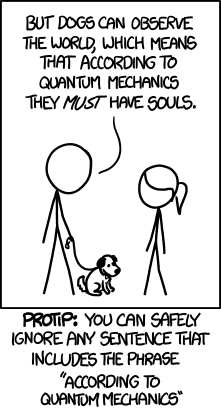
\includegraphics[width=0.27\linewidth]{xkcd-quantum} \label{fig:xkcd1} %\hspace{2cm}
%	\subfloat[]{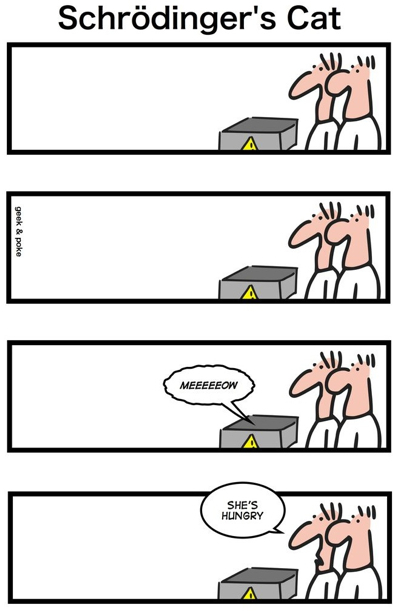
\includegraphics[width=0.33\linewidth]{geek-quantum} \label{fig:geek1}}
	\caption{Image courtesy of \href{https://xkcd.com/1240/}{xkcd}.}
%	\protect\subref{fig:geek1} Image courtesy of \href{http://www.datamation.com/news/tech-comics-quantum-physics-1.html}{Geek and Poke}.}
	\label{fig:comic1}
\end{figure}

In this chapter, we will be tracing through the development of quantum mechanics from its origins, using real experiments to guide our understanding. While the subject of quantum mechanics is often regarded with apprehension and mocked for its complexity (Figure~\ref{fig:comic1}), the examples presented here should reveal how truly fascinating and ubiquitous some of these phenomena are. Let's begin our journey!

%%%%%%%%%%%%%%%%%%%%%%%%%%%%%%%%%%%%%%%%%%%%%%%%%%%%%%%%%%%%%%%%%%%%%%%%%%%%%%%%

\section[Shock treatment]{Shock treatment: The Stern-Gerlach experiment}
Historically, quantum mechanics developed out of a number of experiments performed at the beginning of the 20th century that challenged physicists' notions of how the world works. Today, the bizarre results of these experiments are fundamental to the operation of everyday devices like computers, DVDs, solar cells, and more. And yet, even now, these experiments continue to shock and dazzle us with how weird and unintuitive they seem. As a ``shock treatment'' in quantum mechanics, let us consider the Stern-Gerlach experiment, performed by Otto Stern and Walther Gerlach in 1922.\footnote{For more details on the Stern-Gerlach experiment, check out  \href{http://physicstoday.scitation.org/doi/10.1063/1.1650229}{this article} from \emph{Physics Today} \textbf{56}, 12, 53 (2003).} This experiment, besides illustrating many of the important principles of quantum mechanics, also provides the basis for many other devices and techniques, including magnetic resonance imaging (MRI), lasers, and atomic clocks. \par

\begin{figure}[!h]
	\centering
	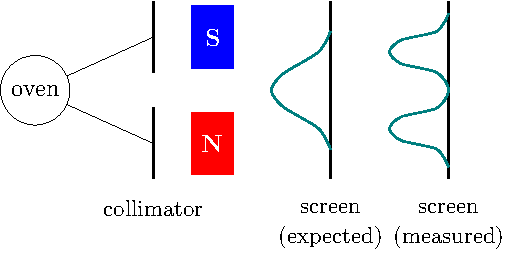
\includegraphics[width=0.5\linewidth]{SG-app}
	\caption{Schematic of the Stern-Gerlach apparatus. An oven releases a beam of silver atoms through a magnetic field, and the resulting distribution that's measured contains two regions of high intensity (second screen).}
	\label{fig:SG-app}
\end{figure}

In this experiment (Figure~\ref{fig:SG-app}), an oven of silver atoms (Ag) is heated to high temperatures, which leads the oven to emit a beam of Ag. This atomic beam is collimated (narrowed) and then sent through a non-uniform magnetic field. Now, atoms have a magnetic dipole moment which is mainly associated with the angular momentum of electrons within the atom. The magnitude and direction of this magnetic moment determine the forces the atom will experience in a magnetic field. A magnetic field oriented along the $z$-axis (pointing to the top of the page) will interact with the $z$ component of the magnetic moment and deflect it by an amount proportional to the magnitude and sign of the magnetic moment. This deflection can be measured by directing the emerging atomic beam onto a screen which detects where the atom hits. Thus, this simple apparatus ``measures'' the $z$ component of the magnetic moment, or alternatively, the $z$ component of the angular momentum. We will label this component $S_z$ and we will call this magnetic field an \textbf{analyzer} since it analyzes the distribution of magnetic moments along the $z$ direction. \par

One expects the Ag atoms to emerge from the oven randomly oriented and thus one would expect to observe on the screen a simple blob showing the broad distribution of orientations. Amazingly, what is observed instead are two discrete components, which seem to imply that there are only two possible values for $S_z$, which we will label as $S_z^+$ and $S_z^-$ corresponding to values which point parallel and antiparallel to the magnetic field respectively. In this way, it appears that angular momentum is quantized, i.e. it does not exhibit a continuum of values but instead only two discrete values. The two regions that are measured on the screen are shown schematically in Figure~\ref{fig:SG-app}. \par

\begin{figure}[!h]
	\centering
	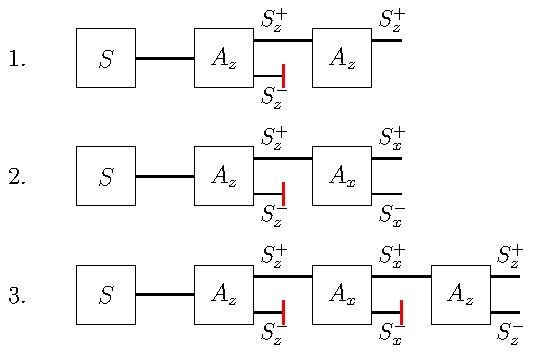
\includegraphics[width=0.5\linewidth]{SG-full}
	\caption{Measurements performed in the Stern-Gerlach experiment. $S$ is the beam source, $A$ is an analyzer, and the subscripts denote the directional orientation.}
	\label{fig:SG-full}
\end{figure}

But this is not the end of the surprises. Consider, as shown in Figure~\ref{fig:SG-full}, the following set of experiments. In the first, the atomic beam is directed from its source $S$ through a $z$-oriented Stern-Gerlach analyzer, labeled $A_z$. From this first analyzer emerges the two components $S_z^+$ and $S_z^-$ which are spatially separated. We then block the $S_z^-$ component and send the $S_z^+$ component into another analyzer $A_z$ also oriented in the $z$ direction. What emerges is only a single component corresponding to $S_z^+$. Makes sense! After all, we have previously blocked the $S_z^-$ component so we would not expect it to appear again. \par

But now consider a variation on this. In the second experiment, we again filter along the $z$ direction and block the $S_z^-$ component before sending the $S_z^+$ component into an analyzer $A_x$ oriented in the $x$ direction. We now again observe only two components emerge, which shows that the magnetic moment is also quantized along the $x$ direction as $S_x^+$ and $S_x^-$. Well, OK, this is at least consistent with the first experiment. Since filtering along $z$ says nothing about the $x$ orientation, it would be reasonable to believe that $A_x$ would still split the remaining beam into two. \par

Finally, consider the third experiment which is the strangest of them all. Here we take the output of the second experiment, block the $S_x^-$ component as shown, and then send the $S_x^+$ component into another $z$-oriented analyzer. What emerges are again two beams $S_z^+$ and $S_z^-$. But we have already blocked the $S_z^-$ component in the first step! And now it has somehow reappeared. It seems as if by measuring along $x$, we have destroyed the information that we thought we knew about the $z$-oriented components. This is often phrased as: One can't measure $S_x$ and $S_z$ simultaneously.\footnote{As groundbreaking as this discovery was, Stern would be nominated 80 times for the Nobel prize before eventually winning the 1943 Nobel Prize in Physics. Gerlach won it the following year. Neither citation mentioned their experiment.} \par

%%%%%%%%%%%%%%%%%%%%%%%%%%%%%%%%%%%%%%%%%%%%%%%%%%%%%%%%%%%%%%%%%%%%%%%%%%%%%%%%

\section{Polarization of light}
The above results should seem quite unusual. But in many ways, these results are similar to what is obtained when one sends light through a series of polarizers. We know that light is a wave and we know that it can be described by an oscillating electric and magnetic field, with a polarization defining the plane in which the electric field oscillation takes place. We performed the following experiments in class (Figure~\ref{fig:polarizer}). First, we take a light source and send it through a polarizer oriented in the $x$ direction, labeled as $P_x$. If we now send the beam through a $y$-oriented polarizer $P_y$, we get nothing out---the beam is completely extinguished as the $x$-oriented light leaving the $P_x$ polarizer is completely absorbed by the orthogonally-oriented $P_y$ polarizer. \par

\begin{figure}[!h]
	\centering
	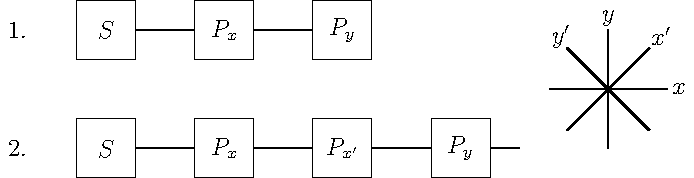
\includegraphics[width=0.6\linewidth]{polarizer}
	\caption{Experiments with light and crossed polarizers. $P_j$ represent polarizers oriented along the $j$ direction. The axes directions are indicated on the right.}
	\label{fig:polarizer}
\end{figure}

But if we now insert in between the $x$ and $y$ polarizers another polarizer oriented in the $x'$ direction, as shown in the diagram, we observe that suddenly, even though we have inserted a filter that can only absorb light, a beam now emerges from the $y$-oriented polarizer. Once again, one could argue that by measuring the beam along the $x'$ direction we have destroyed the information that we thought we had about the polarization after passing through $P_x$. Now, in classes in optics and waves, this is not how one views such a process. Instead, we make use of \textbf{superposition}, in which we think of a wave as being made up of a \emph{sum} of two other waves. Indeed, referring to the axes in Figure~\ref{fig:polarizer}, we may write the state of the $x$ polarized beam in the following way:
\begin{equation}
	\ket{x} = \frac{1}{\sqrt{2}} \left( \ket{x'} - \ket{y'} \right) \label{eq:sup-polar}
\end{equation}
where the notation $\ket{x}$ refers to the state of the $x$ polarized beam.\footnote{This ``bra-ket'' notation is commonly used in quantum mechanics to describe quantum states without the gory details. It will be formally discussed in Section~\ref{sec:braket}.} This equation is just a vector equation---it says that we can associate a vector $\ket{x}$ with the $x$ polarized beam and this equals a vector sum of two other components, namely, $\ket{x'}$ and $\ket{y'}$. The $\frac{1}{\sqrt{2}}$ factor is just a normalization constant to make the length of the vector equal to 1. Similarly, we can write
\begin{equation}
\ket{x'} = \frac{1}{\sqrt{2}} \left( \ket{x} + \ket{y} \right) \label{eq:sup-polar2}
\end{equation}

Viewed in this way, it's not surprising that we get output from the $x'$-oriented polarizer and then subsequently from the $y$-oriented polarizer. After all, the $x$ polarized beam can be thought of as a superposition of an $x'$ and $y'$ polarized beam as described in Equation~\ref{eq:sup-polar}. Thus, the $x'$ oriented polarizer just selects out the $x'$ component. Similarly, the $y$-oriented polarizer just selects out the $y$ component in the $x'$ polarized beam (Equation~\ref{eq:sup-polar2}). \par

From this perspective, the Stern-Gerlach experiment looks very similar to the experiment with light and polarizers. In fact, it's as if we observed \emph{particles behaving as waves}. Furthermore, in direct analogy to the discussion above, we now argue that in the last step of the 3rd experiment described in Figure~\ref{fig:SG-full}, in which a $z$-oriented analyzer probes the $S_x^+$ beam and finds two components $S_z^+$ and $S_z^-$, it must be the case that
\begin{equation*}
	\boxed{\ket{S_x^+} = \frac{1}{\sqrt{2}} \left( \ket{S_z^+} + \ket{S_z^-} \right)}
\end{equation*}

In other words, particles can be in a superposition of two different states at the same time. We will come back to this many times in this course. \par

%%%%%%%%%%%%%%%%%%%%%%%%%%%%%%%%%%%%%%%%%%%%%%%%%%%%%%%%%%%%%%%%%%%%%%%%%%%%%%%%

\section{Wave-particle duality}
We argued above that the silver atoms in some respects are behaving as waves. This dual behavior became known as \textbf{wave-particle duality} and is instrumental in the formulation of quantum mechanics. The theory states that elementary particles (electrons, photons, etc.) can be partly described in terms of particles and partly in terms of waves, with no single concept individually sufficient. As Albert Einstein once said,\footnote{A. Einstein and L. Infeld, \textbf{The Evolution of Physics}, 1938, pg. 262-263.}
\begin{quote}
	``There seems no likelihood for forming a consistent description of the phenomena of light by a choice of only one of the two languages. It seems as though we must use sometimes the one theory and sometimes the other, while at times we may use either. We are faced with a new kind of difficulty. We have two contradictory pictures of reality; separately neither of them fully explains the phenomena of light, but together they do.''
\end{quote}

As the unintuitive nature of the Stern-Gerlach experiment might suggest, scientists took a long time to arrive at this conclusion and they continued to debate its interpretation long after it was formulated.\footnote{See \href{https://en.wikipedia.org/wiki/Interpretations\_of\_quantum\_mechanics}{interpretations of quantum mechanics} on Wikipedia.} Although it's difficult to \emph{exactly} describe quantum-scale behavior, wave-particle duality helps explain a lot of what is found in theoretical and experimental results.

%%%%%%%%%%%%%%%%%%%%%%%%%%%%%%%%%%%%%%%%%%%%%%%%%%%%%%%%%%%%%%%%%%%%%%%%%%%%%%%%

\subsection{Young's double-slit experiment} \label{sec:double-slit}
In the 18th and early 19th century, the prevailing notion, due to the foundations of classical theory and the limits of scientific equipment, was that light behaved as a wave. Early work done by Christiaan Huygens and Augustin-Jean Fresnel on the diffraction of light supported the wave theory. Perhaps one of the most obvious manifestations of light's wave-like behavior is in the appearance of interference patterns, an example being the amazing colors that reflect from oil puddles in the street. \par

\begin{figure}[!h]
	\centering
	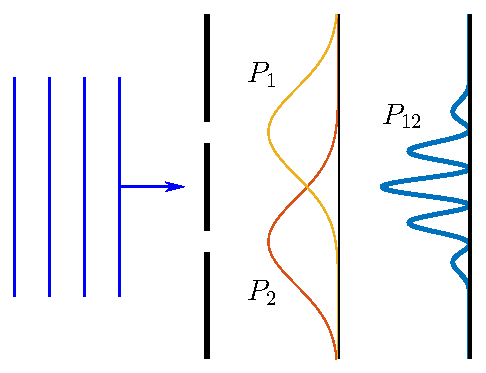
\includegraphics[width=0.5\linewidth]{double-slit}
	\put(-100, -5) {single}
	\put(-40, -5) {interference}
	\put(-240,-5) {plane wave}
	\caption{Schematic of the double-slit experiment. When the plane wave enters the single slits, blobs of intensity are left on the screen. However, a double-slit causes interference between the wavefronts, leaving behind alternating bands of high and low intensity on the screen.}
	\label{fig:double-slit}
\end{figure}

Then, in 1803, Thomas Young's discovery of double-slit interference only seemed to further validate the wave theory and dispel other explanations. Let's consider that experiment, where a plane wave is incident on a double slit as shown in Figure~\ref{fig:double-slit}.\footnote{See this \href{http://micro.magnet.fsu.edu/primer/java/interference/doubleslit/}{interactive tutorial} of the double-slit experiment from Florida State University.} A screen behind the slit measures the light distribution pattern. If only slit 1 is open, we measure a blob behind slit 1, with intensity and distribution $P_1$ as shown. A similar result $P_2$ is observed with only slit 2 open. But if both slits are open, an interference pattern results, corresponding to $P_{12}$. Note that there are some places on the second screen where the intensity is less than when only $P_1$ or $P_2$ are observed, and vice versa. \par

If we try to describe the behavior mathematically, we can associate a wave amplitude due to slit 1 and slit 2 of magnitude $h_1$ and $h_2$ respectively. The intensity patterns are then $P_1=h_1^2$ and $P_2=h_2^2$ for the single-slit case. For the case both slits are open, we have
\begin{equation}
	P_{12} = \abs{h_1+h_2}^2 = \abs{h_1}^2 + \abs{h_2}^2 + 2\abs{h_1}\abs{h_2} \cos \phi  \label{eq:interf}
\end{equation}
where $\phi$ is the phase difference between the two waves. This equation clearly shows the emergence of an interference term and supports the theory of continuous, wave-like behavior. \par

%%%%%%%%%%%%%%%%%%%%%%%%%%%%%%%%%%%%%%%%%%%%%%%%%%%%%%%%%%%%%%%%%%%%%%%%%%%%%%%%

\subsection{Photoelectric effect}
While the wave theory of light prevailed for over a century, it was challenged in the early 1900s by two physicists named Max Planck and Albert Einstein. In his work on blackbody radiation, which is the emission of electromagnetic radiation due to heat, Max Planck realized that the physics could only be explained if the energy was \textbf{quantized}; that is, light must be made up of packets (quanta) of energy that varied linearly with frequency ($\nu$, lower-case ``nu'') according to
\begin{equation}
	E = h\nu \label{eq:planck}
\end{equation}
where $h$ is \textbf{Planck's constant}, equal to \SI{6.626e-34}{\joule \cdot \second}. While this explained the physics quite well, Planck thought his idea of ``quanta'' was a limitation of his model and the scientific community did not initially accept his findings.\footnote{His discovery was eventually accepted and Planck was awarded the 1918 Nobel Prize in Physics.} \par

Shortly thereafter in 1905, Albert Einstein used Planck's quantized model of light to explain the photoelectric effect, which renewed the debate over the behavior of light. In the photoelectric effect (Figure~\ref{fig:PE-eff}), photons that strike certain metal surfaces will knock electrons out of the metal and cause current to flow. The strength of the current then, Einstein assumed, should be proportional to the strength of light hitting the surface, which classical theory predicted was proportional to the intensity or amplitude of the light wave. However, what Einstein found was that a dim blue light was capable of ejecting electrons, but that a red light was not---no matter how bright or shown for how long. Therefore, he reasoned that a beam of light was composed of discrete wave packets (\textbf{photons}) that each had an energy according to Equation~\ref{eq:planck}. The explanation Einstein offered for the photoelectric effect was so instrumental to the development of quantum mechanics that he was awarded the 1921 Nobel Prize in Physics for this discovery.\footnote{For a translation of Einstein's original work, see \href{http://astro1.panet.utoledo.edu/~ljc/PE\_eng.pdf}{this document} courtesy of the University of Toledo.}$^,$\footnote{See \href{https://www.scientificamerican.com/article/einstein-s-legacy-the-photoelectric-effect/}{this article and podcast} on the photoelectric effect from Everyday Einstein, \emph{Scientific American}, 18 Aug 2015.}
\begin{figure}[!h]
	\centering
	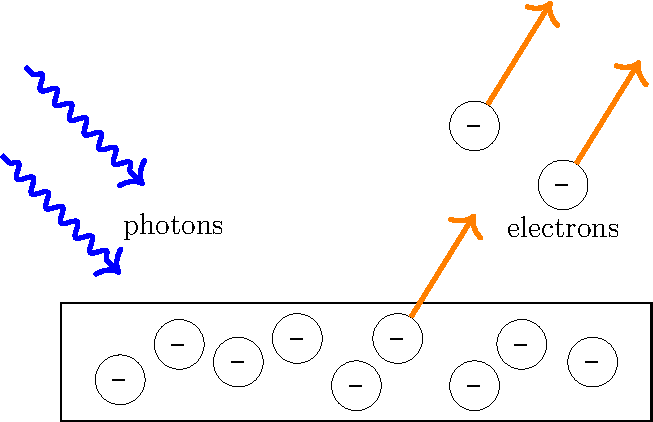
\includegraphics[width=0.5\linewidth]{photoelectric-effect}
	\caption{Schematic of the photoelectric effect, whereby electrons are emitted when light shines on a material. Adapted from \href{https://en.wikipedia.org/wiki/Photoelectric\_effect}{Wikipedia}.}
	\label{fig:PE-eff}
\end{figure}

%%%%%%%%%%%%%%%%%%%%%%%%%%%%%%%%%%%%%%%%%%%%%%%%%%%%%%%%%%%%%%%%%%%%%%%%%%%%%%%%

\subsection{De Broglie hypothesis} \label{sec:db-hyp}
Einstein's discovery had profound consequences, as it appeared to give indisputable evidence that light had both particle-like and wave-like characteristics. This naturally led scientists to ask the following question: Do all matter behave as such? That is, even though we think of electrons and atoms as particles, could they also display wave-like behavior? \par

In 1924, Louis de Broglie, for his PhD thesis, decided to take the findings from Planck and Einstein and associate a frequency and wavelength with all types of matter. Recall that Einstein had already showed, in his interpretation of the photoelectric effect, that photons have energy given by
\begin{tcolorbox}[title=Energy relationship] \vspace{-2ex}
	\begin{equation}
		E = h\nu = \hbar \omega \label{eq:EdB}
	\end{equation}
\end{tcolorbox}

where $\hbar$ is the \textbf{reduced Planck's constant} equal to $\frac{h}{2\pi}$ and $\omega$ is angular frequency equal to $2\pi\nu$. We can also derive an equation for momentum, given by
\begin{tcolorbox}[title=Momentum relationship] \vspace{-2ex}
	\begin{equation}
		p = mc = \frac{E}{c} = \frac{\hbar\omega}{c} = \frac{2\pi\hbar}{\lambda} = \hbar k \label{eq:pdB}
	\end{equation}
\end{tcolorbox}

where $m$ is mass, $c$ is the speed of light, $E$ is energy, and $k=\frac{2\pi}{\lambda}$ is the \textbf{wavenumber}, which is the magnitude of the \textbf{wave vector}. Generally speaking, the wavenumber represents the spatial frequency of a wave, which in this context is the number of radians per unit distance. You can think of it as the number of cycles of the wave in \SI{1}{\meter} of space. \par

In his thesis, de Broglie extended this definition, along with Equations~\ref{eq:EdB} and \ref{eq:pdB}, to describe \emph{all} types of matter. All matter, not just light, display wave-like behavior and have a characteristic de Broglie wavelength $\lambda$ given by
\begin{tcolorbox}[title=de Broglie wavelength] \vspace{-2ex}
	\begin{equation}
		p = \hbar k = \frac{h}{\lambda} \implies \lambda = \frac{h}{p} \label{dBw}
	\end{equation}
\end{tcolorbox}

This was a bold hypothesis that unified the conversations around wave-particle duality and earned Louis de Broglie the 1929 Nobel Prize in Physics (if you haven't caught on yet, quantum mechanics is a big deal). Of course, in a classic case of ``don't believe it till you see it,'' scientists had to first figure out a way to experimentally verify this hypothesis.

%%%%%%%%%%%%%%%%%%%%%%%%%%%%%%%%%%%%%%%%%%%%%%%%%%%%%%%%%%%%%%%%%%%%%%%%%%%%%%%%

\subsection{Davisson-Germer experiment}
Between the years of 1923 and 1927, Clinton Davisson and Lester Germer performed a series of experiments at Bell Labs that (incidentally) confirmed the de Broglie hypothesis.\footnote{See \href{https://physics.aps.org/story/v17/st17}{this article} in \emph{APS Physics} for details on the Davisson-Germer experiment and the original papers.} In their experiment, Davisson and Germer placed an electron gun and nickel (Ni) target inside a high vacuum chamber (see Figure~\ref{fig:DG}). The electron gun emitted a beam of electrons incident on the Ni surface and a detector was used to capture the scattered electrons. What surprised the two of them was that the resulting spectra was not uniform and instead featured intense peaks at distinct angles, similar to what Bragg had previously discovered with X-ray diffraction.\footnote{For an interesting read on the discovery of X-ray diffraction, see M. Eckert, \href{http://onlinelibrary.wiley.com/doi/10.1002/andp.201200724/full}{\emph{Annalen der Physik}}, \textbf{524}, A83 (2012).} \par

\begin{figure}[!h]
	\centering
	\subfloat[]{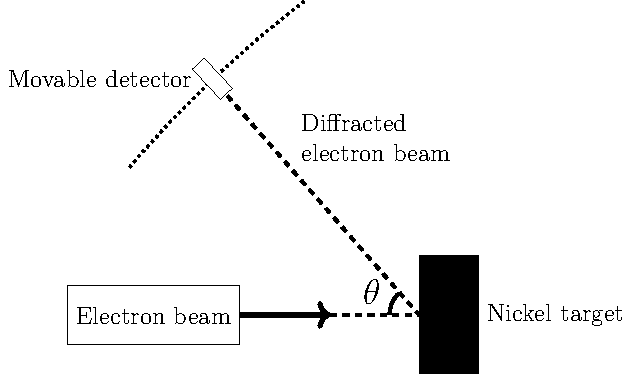
\includegraphics[width=0.5\linewidth]{davisson-germer} \label{DG-exp}}
	\subfloat[]{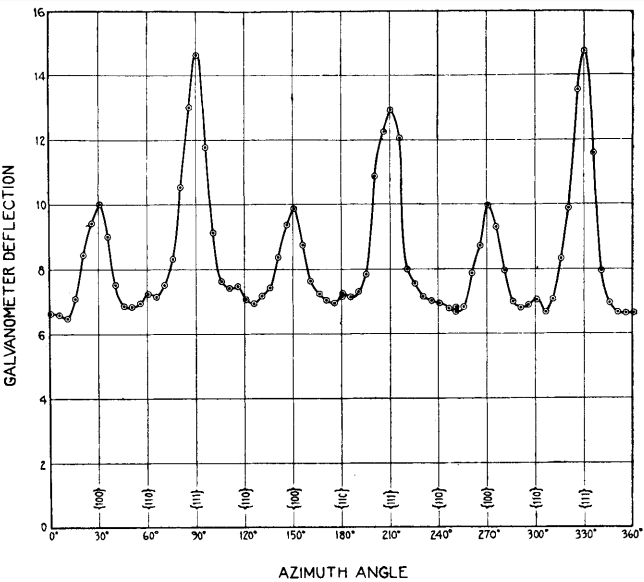
\includegraphics[width=0.5\linewidth]{DG-plot} \label{DG-plot}}
	\caption{\protect\subref{DG-exp} Schematic of the Davisson-Germer experiment. The electron beam scatters from the nickel surface and enters the detector. Adapted from \href{https://en.wikipedia.org/wiki/Davisson\%E2\%80\%93Germer\_experiment}{Wikipedia}. \protect\subref{DG-plot} The spectra contains sharp peaks of intensity at distinct diffraction angles. Reproduced from C. Davisson and L. Germer, \href{https://www.nature.com/nature/journal/v119/n2998/pdf/119558a0.pdf}{\emph{Nature} (London)}, \textbf{119}, 558 (1927).}
	\label{fig:DG}
\end{figure}

The two scientists applied Bragg's law, which states 

\begin{tcolorbox}[title=Bragg's law] \vspace{-2ex}
	\begin{equation}
		n\lambda = 2d\sin\theta \label{eq:bragg}
	\end{equation}
\end{tcolorbox}

where $n$ represents an integer order usually equal to 1, $\lambda$ is the wavelength, $d$ is the spacing between the lattice planes, and $\theta$ is the angle of diffraction. They calculated the wavelength of the diffracted beam given the measured angle and inter-planar spacing of Ni, and found good agreement between their physical observations and theoretical calculations based on de Broglie's hypothesis. Davisson and Germer's discovery was the first direct evidence for the wave-like nature of particles and confirmed the de Broglie hypothesis. And yes, sure enough, Davisson was awarded the 1937 Nobel Prize in Physics for this achievement.\footnote{But \href{http://www.nobelprize.org/nobel\_prizes/physics/laureates/1937/press.html}{where was Germer}?}

%%%%%%%%%%%%%%%%%%%%%%%%%%%%%%%%%%%%%%%%%%%%%%%%%%%%%%%%%%%%%%%%%%%%%%%%%%%%%%%%

\section{Application: Quantum eraser}
Although some of these experiments are over a century old, they established the fundamental basis for more advanced theories and experiments that are still being investigated today. Consider the \textbf{quantum eraser experiment}, which is a variation on Thomas Young's classic double-slit experiment (we saw this in Section~\ref{sec:double-slit}). This experiment was first proposed by Scully et al. in 1991,\footnote{M. O. Scully, B. G. Englert, and H. Walther, \href{https://www.nature.com/nature/journal/v351/n6322/abs/351111a0.html}{\emph{Nature} (London)}, \textbf{351}, 111 (1991).} and a variation on the original design is shown in Figure~\ref{fig:QE}. As we've seen before, the double-slit experiment produces an interference pattern when we send a beam of light through the two slits; however, if we were to reduce the intensity of the light, even to the point where only \emph{single photons} are approaching the two slits, we would \emph{still} see an interference pattern on the screen. This seems to suggest that each photon passing through the slits interferes with itself as if it somehow goes through both slits at once. Indeed, if we then block one of the slits, or somehow mark them to indicate which slit the photon went through, then the interference pattern disappears and the photons behave like classical particles again. \par

\begin{figure}[!h]
	\centering
	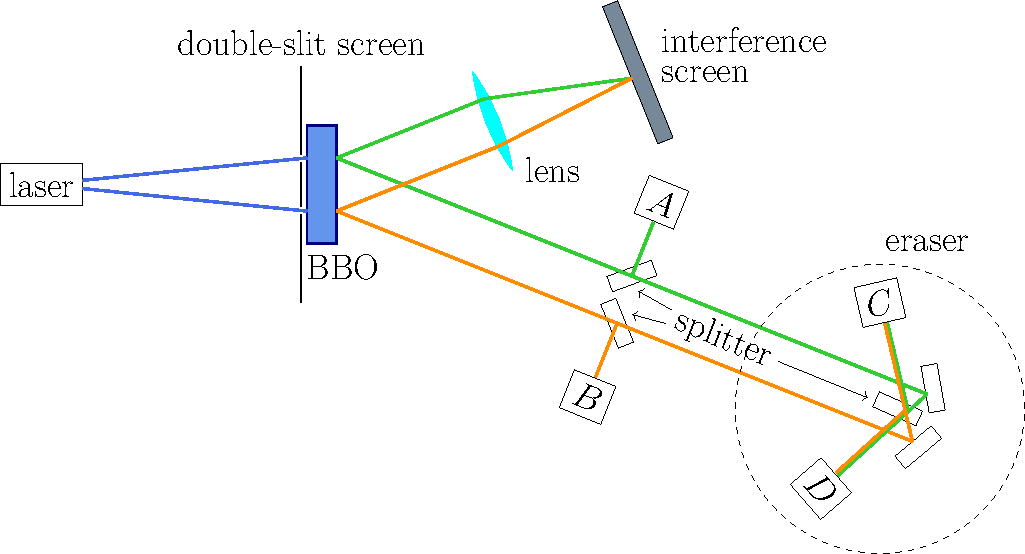
\includegraphics[width=0.6\linewidth]{quantum-eraser}
	\caption{Schematic of the quantum eraser experiment. The BBO crystal splits the single-photon beam into an entangled pair of identical photons. If we make a measurement at the detectors and reveal the origin of one photon, then the interference pattern caused by its twin is destroyed. However, if this information is subsequently ``erased,'' the interference pattern reappears. Adapted from \href{http://www.pbs.org/video/2365862119/}{PBS Space Time}.}
	%Walborn et al., \href{https://journals.aps.org/pra/abstract/10.1103/PhysRevA.65.033818}{\emph{Phys. Rev. A}}, \textbf{65}, 033818 (2002).}
	\label{fig:QE}
\end{figure}

But what would happen if we first marked the slits, and then ``erased'' the markings? If we obscured our knowledge of the path of the photons, even though the photons have already passed through the double slits, would the interference pattern reappear? This is the question investigated by the \textbf{delayed choice quantum eraser}.\footnote{Y. H. Kim et al. \href{https://journals.aps.org/prl/abstract/10.1103/PhysRevLett.84.1}{\emph{Phys. Rev. Lett.}}, \textbf{84}, 1 (2000).} As seen in Figure~\ref{fig:QE}, a laser emits photons toward a double-slit screen, behind which sits a crystal of beta barium borate (BBO). The BBO crystal is able to take a single photon and produce a coherent \textbf{entangled pair} of photons that are identical to each other, allowing us to use the measurements from one photon to determine the state of the other.\footnote{See Section~\ref{sec:further} for more information on quantum entanglement.} One of the entangled photons is sent towards the lens and screen, while the other is sent towards the detectors. If we look at detectors $A$ and $B$, whenever one of them detects a photon (``lights up''), we will know which of the two slits the entangled pair originated from, and this knowledge destroys the interference pattern on the screen. What's more surprising is that even if the other photon hits the screen first, and \emph{then} the first set of detectors light up (i.e. they are placed much farther away than the screen), the interference pattern is still destroyed. It would appear as if our knowledge of where the photon lands on the detectors is capable of retroactively influencing the state of the photon in the past! \par

This is starting to get pretty crazy, but let's take it one step further. We arrange another set of mirrors, splitters, and detectors behind the first set to perform the actual ``erasing.'' Our splitters are half-silvered mirrors that reflect half of the photons that strike them and let the other half pass through. Now if we look at the entangled photons that reach this eraser, they will be equally likely to end up in detector $C$ or $D$, no matter which slit they originally passed through. Accordingly, when we look at their entangled twins on the interference screen, the interference pattern appears again! So, even though we could have figured out exactly which slit the photon came through, obfuscating this information resulted in the photon producing an interference pattern that suggests it passed through both slits at once. \par

This experiment is yet another demonstration of the superposition principle and wave-particle duality that we previously discussed. As it turns out, wave-particle duality is a special case of a more general principle in quantum mechanics known as \textbf{complementarity}. This principle states that complementary properties of objects (e.g. wave-like and particle-like behavior) cannot be measured simultaneously. We will certainly see this principle again in the near future.

%%%%%%%%%%%%%%%%%%%%%%%%%%%%%%%%%%%%%%%%%%%%%%%%%%%%%%%%%%%%%%%%%%%%%%%%%%%%%%%%

\section{Summary}
Congratulations on making it through the first chapter! To recap, we traced the development of quantum mechanics in the 19th and 20th century and got a glimpse into some of the brilliant minds that established this field. Understanding the intellectual history of quantum mechanics not only acknowledges the contributions made by others, but also helps us build intuition about these mind-boggling concepts. We first saw scientists like Young, Planck, and Einstein propose wave-like and particle-like behavior for light. Then de Broglie introduced his groundbreaking hypothesis of wave-particle duality, which was later confirmed by Davisson and Germer in their experiments. We began the chapter with the Stern-Gerlach experiment, which also occurred around the same time and demonstrated the fundamental wave principle of superposition, and we concluded with a modern application in the quantum eraser experiment. \par

This chapter was filled with some pretty dense and unintuitive material---accordingly, you should view the examples less as something that requires complete understanding for now and more as motivation for what's to come. While having some classical physics intuition is good, quantum mechanics often has a mind of its own, so it will be a little uncomfortable as you adjust yourself to this new way of thinking. Examples are an excellent, concrete way to demonstrate theoretical principles, but eventually we will need to have a mathematical description for these phenomena. This is the topic of the next chapter as we look at the contributions of Erwin \Sch\ and his famous wave equation.

%} % for doublespacing
%\end{document}
